\documentclass[]{article}
\usepackage[letterpaper, margin=1in]{geometry}
\usepackage{setspace}
\usepackage{graphicx}
\usepackage{lineno}
\usepackage{multirow}
\usepackage{placeins}
\usepackage{float}
\usepackage{caption}
\graphicspath{{../Figures/}}
\usepackage{gensymb}
\doublespacing
\usepackage{amsmath, amssymb} % Math packages
\usepackage{amsthm}
\usepackage{natbib}
\setlength{\parindent}{0cm}

\begin{document}


\section{Simulation Study}

We compare the performance of our quantile trend filtering method with the three previously published methods using designs proposed by \cite{Racine2017}. The methods compared are 

\begin{itemize}
	\item \texttt{npqw}: \cite{Racine2017} constrain the response to follow a smooth location scale model of the form $Y_i = a(X_i) + b(X_i)\epsilon_i$. They estimate the $\tau$\textsubscript{th} conditional quantile given $X_i = x$ using a kernel estimator
	\begin{equation}
		q_{\tau}(x) = \frac{\sum_{i=1}^n \Phi^{-1}_{(Y_i, b(X_i))}(\delta_0)K_h(X_i,x)}{\sum_{i=1}^nK_h(X_i, x)}
	\end{equation}
	defining $\Phi^{-1}_{(Y_i, b(X_i))}(\delta_0)$ as the quantile function of the Normal distribution with mean $Y_i$ and standard deviation $b(X_i)$ evaluated at $\tau$. $\delta_0$ is a function of $\tau$ and chosen empirically, $h$ is a tuning parameter and $K$ is a kernel function. Code was obtained from the author for the \texttt{quantile-ll} method. 
	
	\item \texttt{qsreg}: \cite{Oh2011} proposed a pseudo-data algorithm for a quantile spline estimator of the form 
	\begin{equation}
	\sum_i \rho_{\tau}(y_i - g(x_i)) + \lambda\int(g''(x))^2dx.
	\end{equation} 
	If $\rho_{\tau}(\cdot)$ were differentiable, the solution to this equation would take a form similar to that of the squared loss smoothing spline with weights equal to $\frac{\rho'_{\tau}(y_i-g(x_i))}{2(y_i - g(x_i))}$. Relying on this idea, Nychka proposed to solve the problem by iteratively solving the weighted smoothing spline. To address the non-differentiability they propose an approximation 
	\begin{equation}
	\rho_{\tau, \delta}(u) = [\tau I(u>0) + (1-\alpha)I(u<0)]u^2/\delta
	\end{equation}
	The function \texttt{qsreg} in the \texttt{fields} R package was used. The smoothing parameter is chosen automatically using generalized cross validation on the pseudo data.
	
	\item \texttt{rqss}: \cite{KoenkerNgPortnoy1994} Koenker proposed smoothing splines using trend filtering with the second order differencing matrix which results in linear splines. The function \texttt{rqss} in the \texttt{quantreg} package implements this method. The smoothing parameter $\lambda$ is chosen using a grid search and minimizing 
	\begin{equation}
	SIC(p_{\lambda}) = log[n^{-1}\sum\rho_{\tau}(y_i - \widehat{g}(x_i))] + \frac{1}{2n}p_{\lambda}log n
	\end{equation}
	where $p_{\lambda} = \sum I(y_i = \widehat{g}_i(x_i))$, which can be thought of as active knots.
	
	\item \texttt{detrendr\_SIC}: Our method where we minimize
	$\sum_i\rho_{\tau}(y_i - \theta_i) + \lambda||D\theta||_1$ and $\lambda$ is chosen using SIC from above. A single value of $\lambda$ was chosen by scaling and summing SIC values across all quantiles. 
	\item \texttt{detrendr\_valid}: Our method where lambda is chosen by leaving out every 5th observation as a validation data set and evaluating the check loss function on the validation data. 
\end{itemize}

Three simulation designs from \cite{Racine2017} were considered. For all designs $X_i$ was generated as a uniformly spaced sequence in $[0,1]$ and the response $Y$ was generated as 
$$Y_i = sin(2\pi x_i) + \epsilon_i(x_i)$$
The three error distributions considered were 
\begin{itemize}
 \item Gaussian: $\epsilon_i(x_i) \sim N\left(0, \left(\frac{1+x_i^2}{4}\right)^2\right)$
 \item Beta: $\epsilon_i \sim Beta(1, 11-10x_i)$
\item Mixed normal: $\epsilon_i$ is simulated from a mixture of $N(-1,1)$ and  $N(1,1)$ with mixing probability $x_i$.
\end{itemize}
\begin{figure}
\caption{Simulated data with true quantiles $\tau \in \{0.01, 0.05, 0.25, 0.5, .75, 0.95, 0.99\}$}	
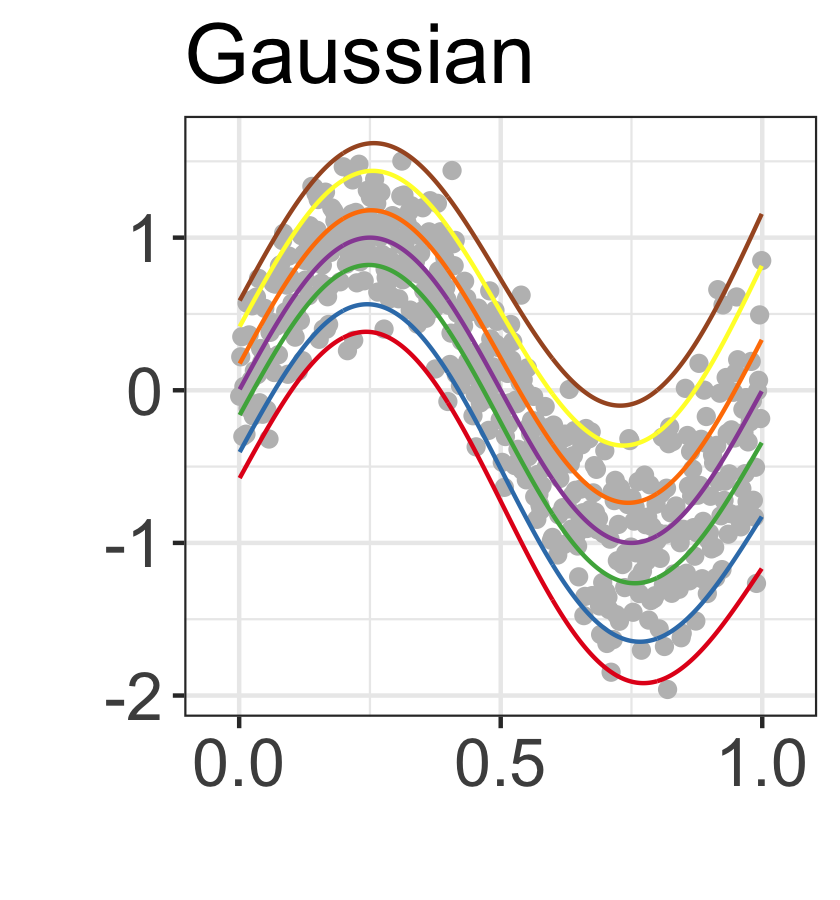
\includegraphics[width=.3\linewidth]{Figures/gaus.png}
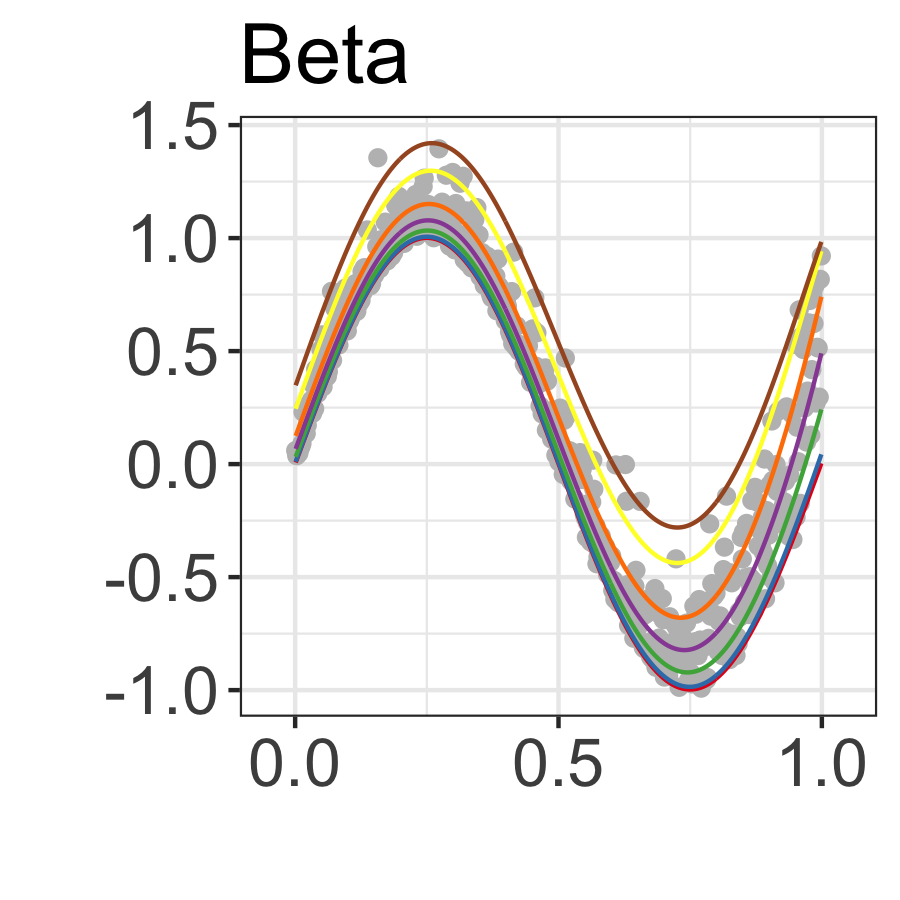
\includegraphics[width=.3\linewidth]{Figures/shapebeta.png}
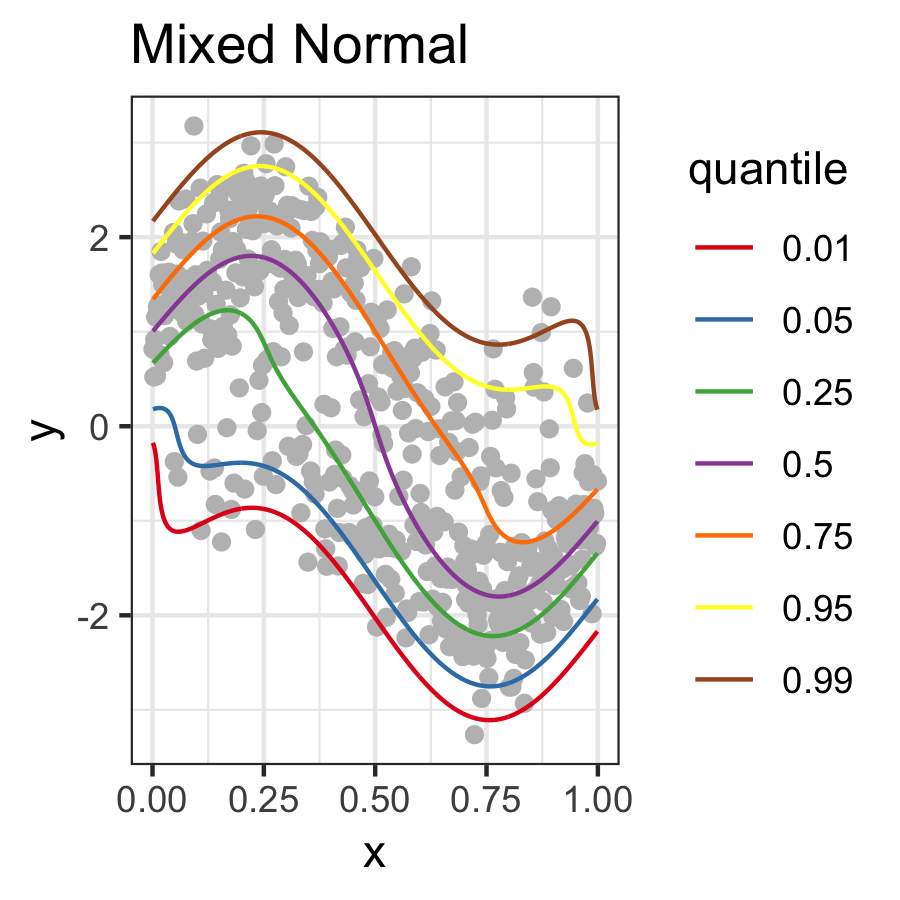
\includegraphics[width=.3\linewidth]{Figures/mixednorm.png}
\end{figure}

100 datasets were generated of sizes 300, 500 and 1000. The MSE was calculated as $\frac{1}{n}\sum_i (\hat{q}_{\tau}(x_i) - q_\tau(x_i))^2$. The plots below show the mean MSE $\pm$ twice the standard error by method, quantile level and sample size. 
	 
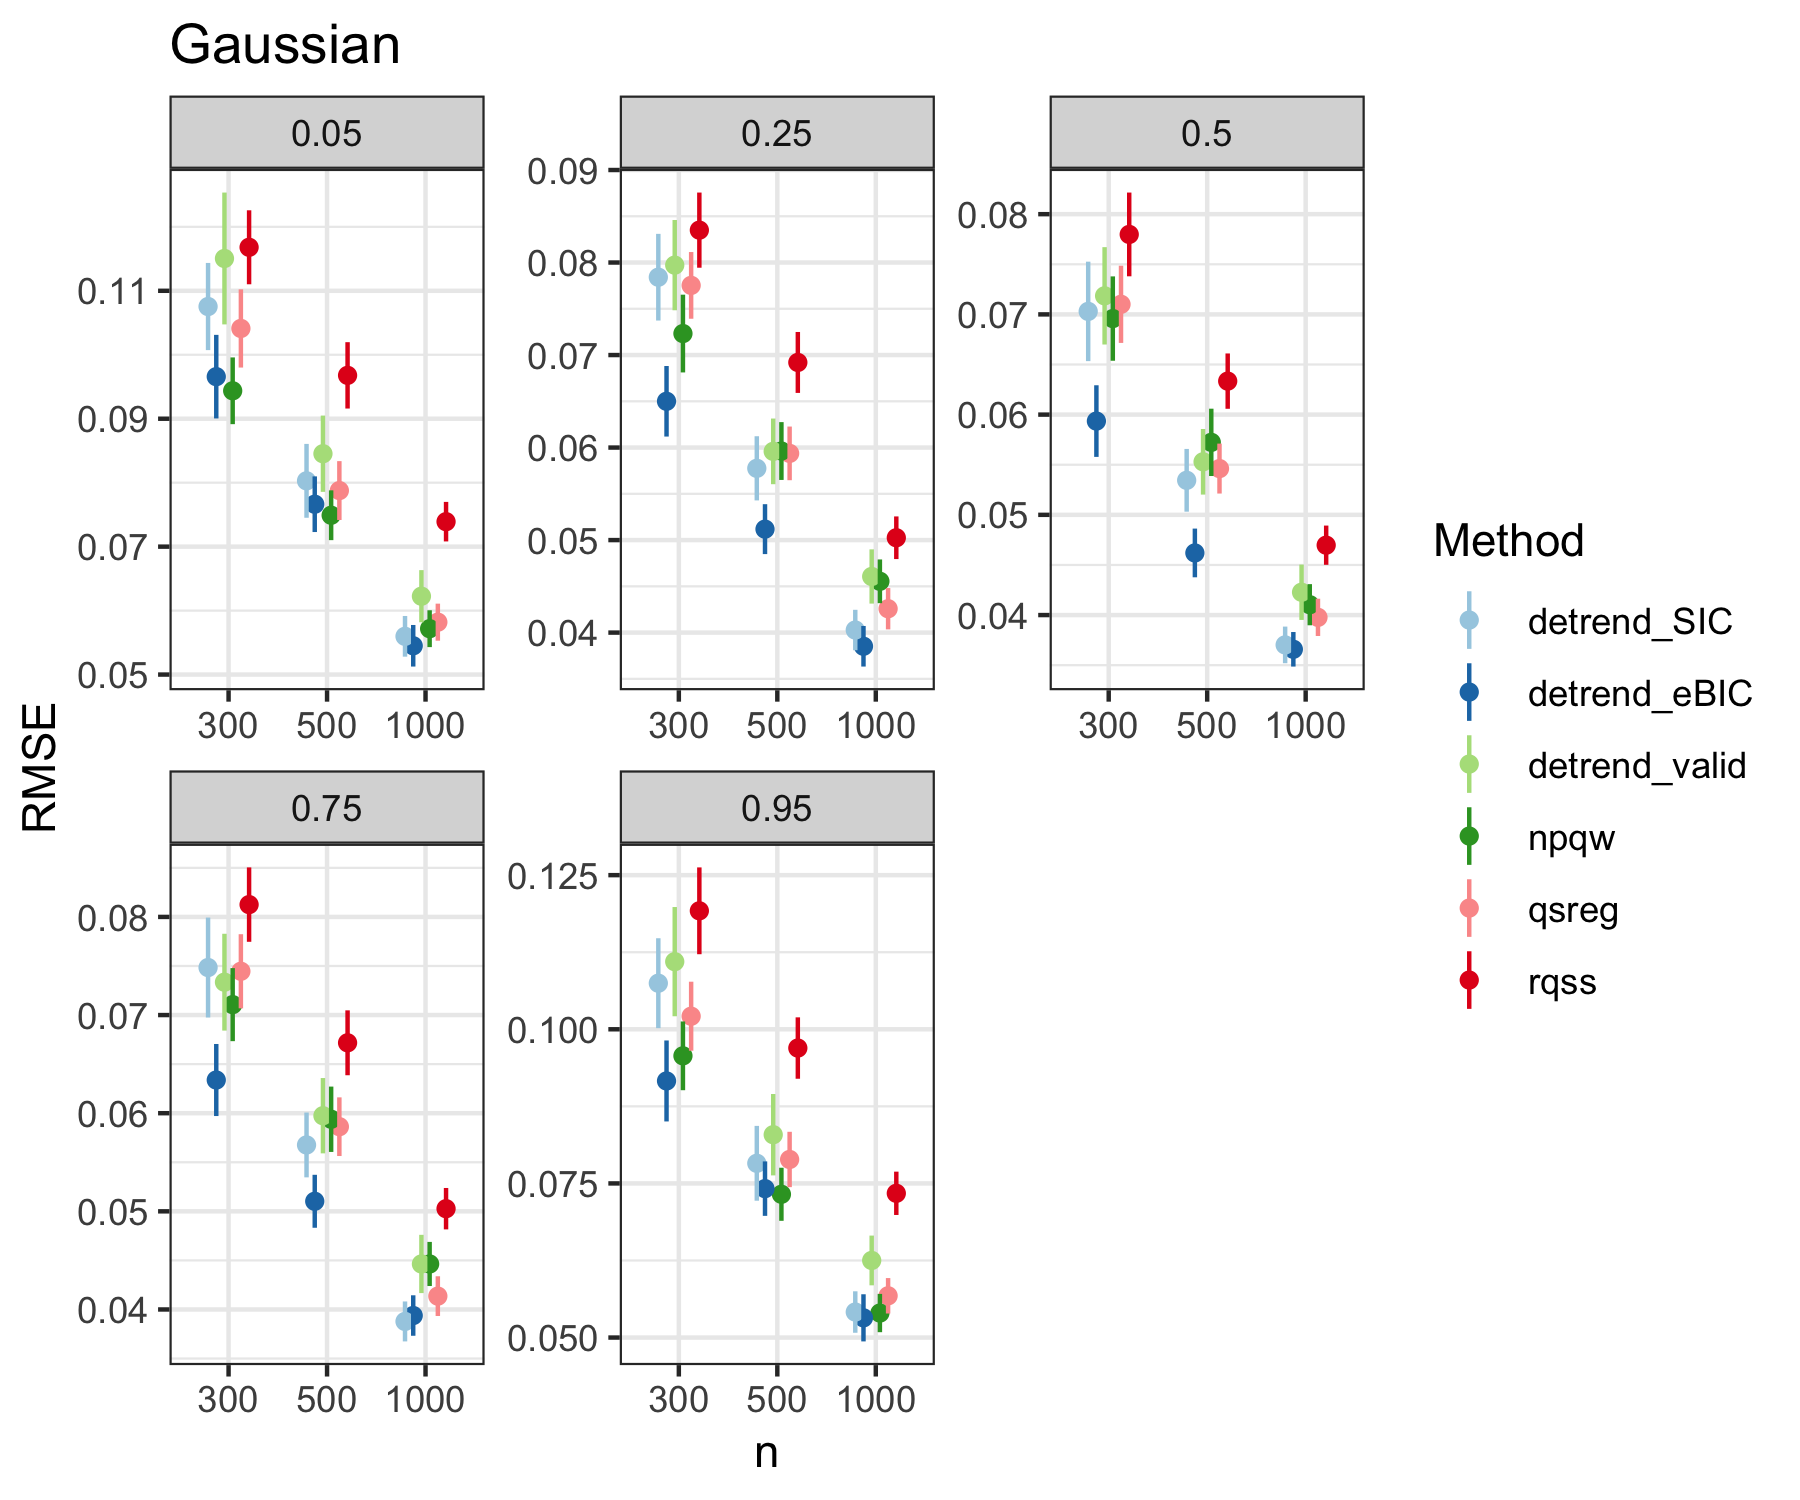
\includegraphics[width=\linewidth]{Figures/gaus_mse.png}	

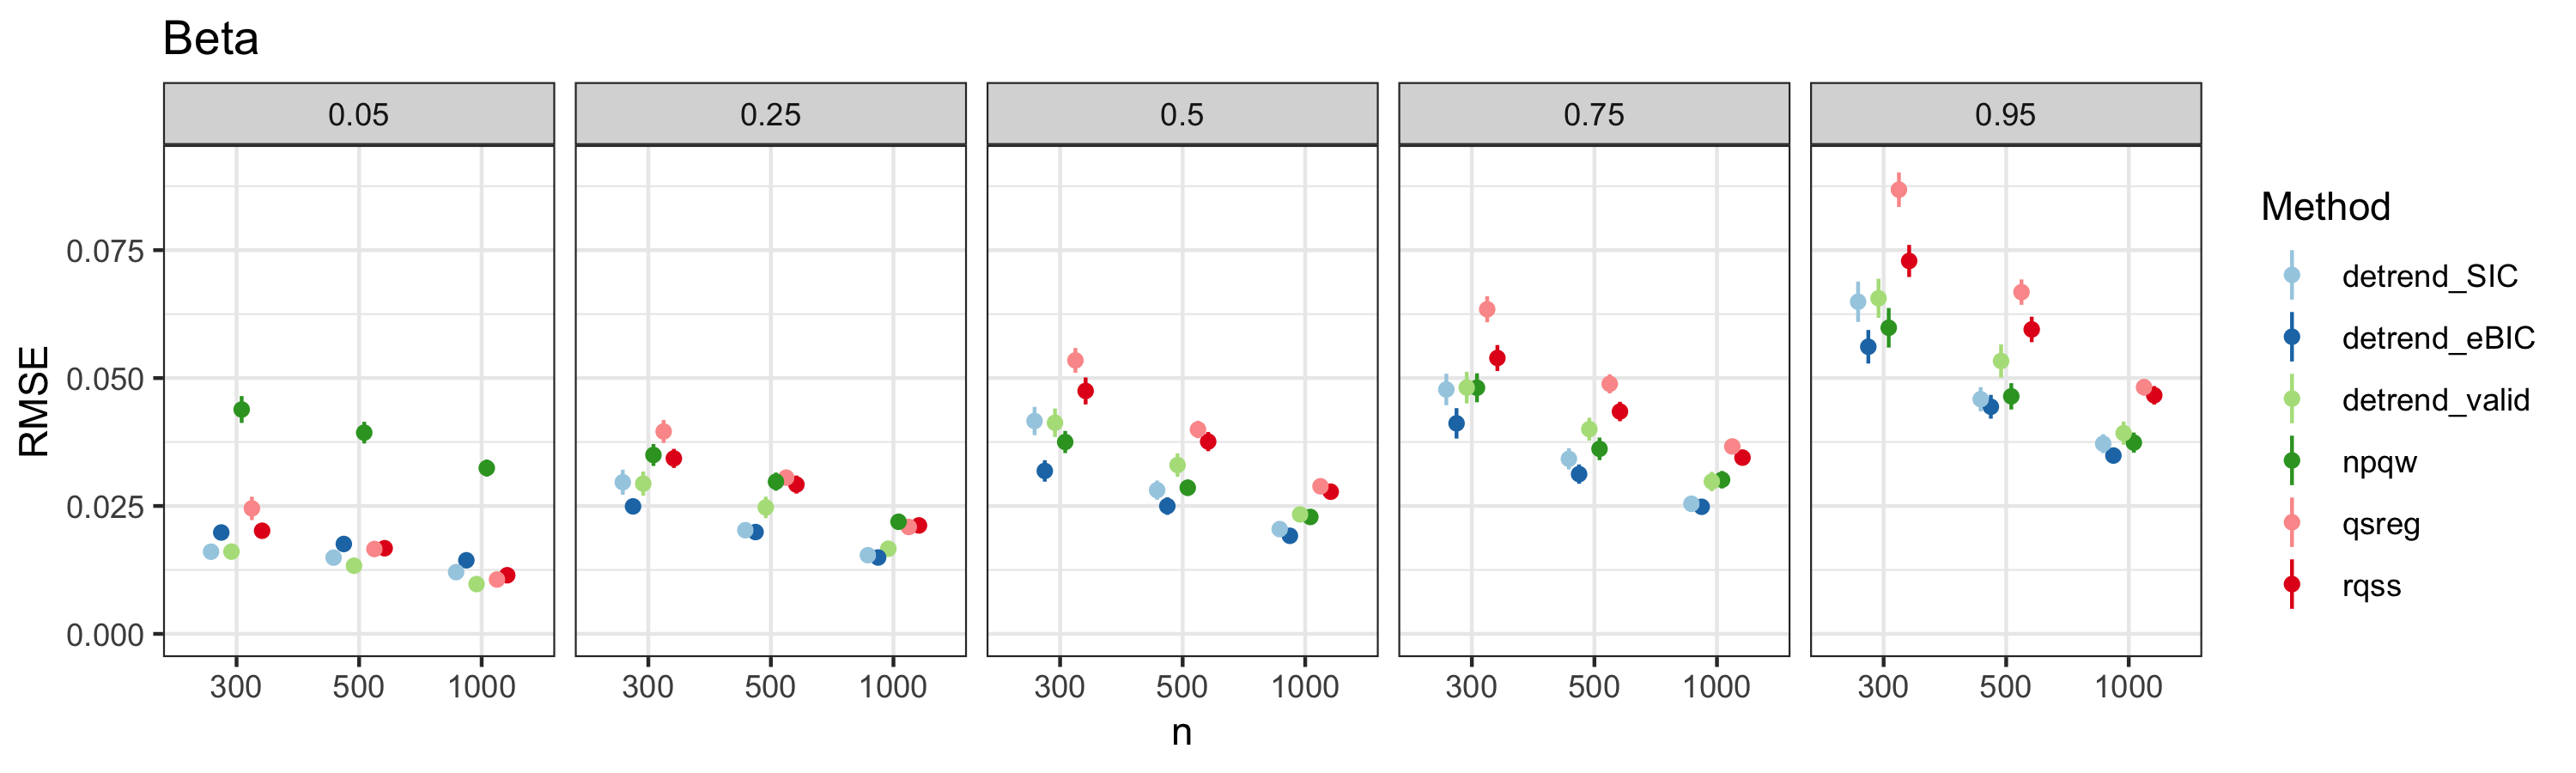
\includegraphics[width=\linewidth]{Figures/shapebeta_mse.png}

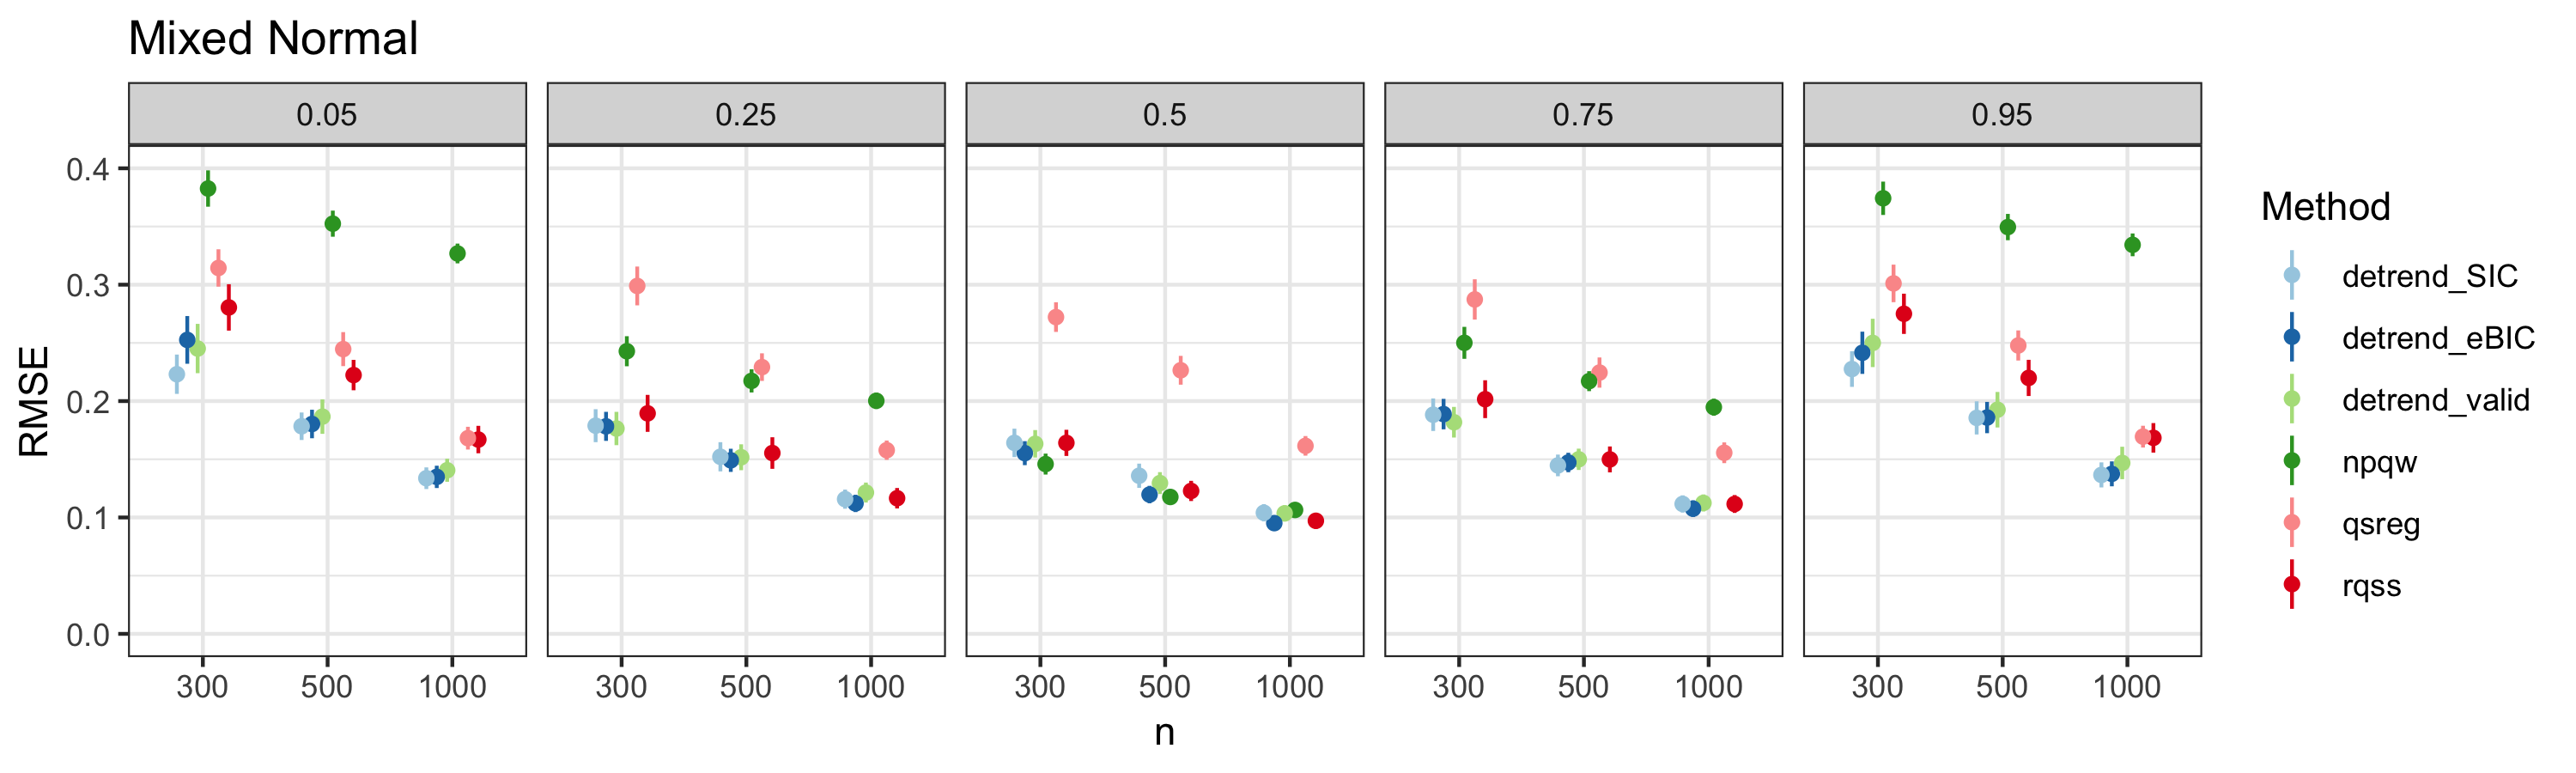
\includegraphics[width=\linewidth]{Figures/mixednorm_mse.png}
\bibliographystyle{asa}
\bibliography{detrendify}
	

\end{document}